\newpage
\subsection*{Question 4}

\begin{enumerate}[label={(\alph*)}]
    \item The table resulting form the insertion of above records is shown bellow:
        \begin{center}
            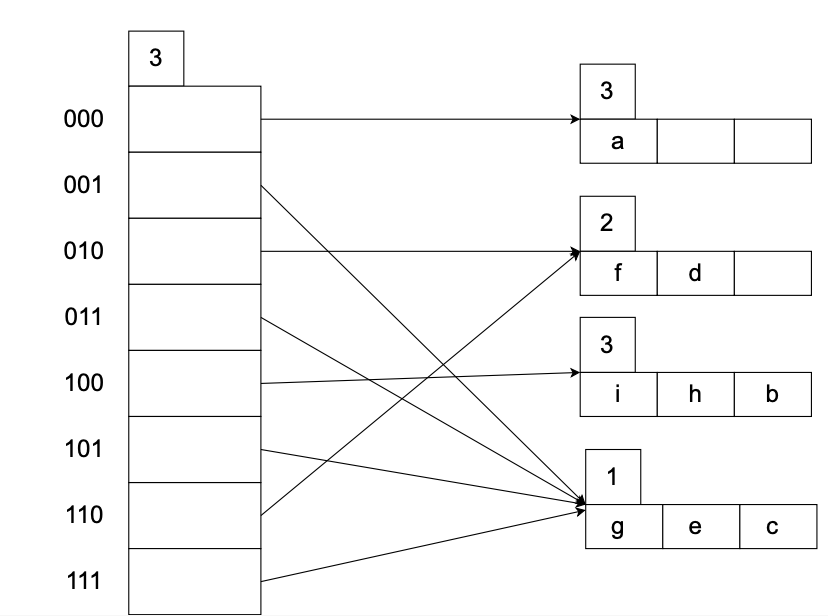
\includegraphics[width=0.9\textwidth]{img/img2.png}
        \end{center}
    
    \item The global depth is 3.
    
    \item There will be 4 buckets.
    
    \item i, h, and b. The bucket has a local depth of 3.
    
    \item g, e, and c. The bucket has a local depth of 1. 
    
    \item \textbf{a)}. The number of bits to be used in the hash function are kept in the global depth.
    
    \item No.
    
    \item If the local depth of a bucket is equal to the global depth of the directory, then the bucket is pointed to by exactly one directory entry. 
\end{enumerate}